\chapter{Governing parameters of fluid-elastic galloping}
\label{chap:pi_1_pi2}
\section{Introduction}

The review of published literature reveals that fluid-elastic galloping has a potential to be used as a mechanism for energy extraction \citep{Barrero-Gil2010a}. Thus, the following questions emerge. What are the optimum parameters for energy transfer in a galloping system? How do they influence galloping?

Another fluid-structure interaction phenomenon, vortex-induced vibration (VIV), has also been investigated as a candidate for the power extraction from flows. The work from \citet{Bernitsas2008a-concept, Bernitsas2009, Raghavan2010a, Lee2011b} and others from the same group at the University of Michigan have made significant progress with this problem. Therefore it may seem, at least initially, reasonable to present data from the fluid-elastic problem in the same parameters as typically used in VIV studies, which could be observed in current literature on galloping \citep{Barrero-Gil2009,Barrero-Gil2010a,Parkinson1964}.



However, the data presented in the pioneering study on energy harvesting from galloping  \citep{Barrero-Gil2010a} presented using classical VIV parameters (i.e. \ustar, $\mstar\zeta$), shows that the mean power data does not collapse well. Here it is hypothesized that the reason behind this is the difference in time-scales of VIV and galloping. Thus the work presented in this chapter is focused on testing this hypothesis. First, new parameters considering this difference in timescale are obtained, and then the optimum conditions for mean power output in terms of these new parameters are found. 

Since the the Quasi-steady state model is the primary mathematical model used to model galloping in this study, the fluid-dynamic characteristics of flow over a static body are presented and discussed first as it is the main input to the QSS model. Then, the natural time scales of the system are obtained using the linearised QSS model. Next, the new non-dimensional governing parameters  \massstiff\ ( a type of combined mass-stiffness) and \massdamp (a combined mass-damping), are formulated by non-dimensionalising the QSS model from these natural time scales. Following this is a comparison of galloping data using the classical VIV parameters and the new parameters \massstiff\ and \massdamp. Then, the influence of \massstiff \ and \massdamp \ and the conditions for an optimum power output are discussed from QSS data. Finally, the QSS data are compared and discussed against FSI direct numerical simulations and final conclusions are presented.

\subsection{Static body results}

The main data acquisition tool for galloping is the QSS model. As discussed in chapter \ref{sec:QSS_model_methodology}, the input to the QSS model is the lift force as a function of the induced angle of attack $\theta$. This function is obtained using lift and drag ($C_y$) data from static body simulations or experiments, to which a polynomial is fitted. These static body data and the polynomial coefficients are presented here in figure \ref{fig:lift_curves} and table \ref{table:cy-coefficients} respectively.  Figure \ref{fig:lift_curves} shows the plots of time averaged $C_y$ data as a function of $\theta$, as well as the $7^{th}$ order polynomial fits. Data were acquired for high and low Reynolds numbers. For high Reynolds numbers, the static body polynomial data are obtained from \cite{Parkinson1964} while for low Reynolds numbers a $7^{th}$ order non-linear least square regression fit on static body DNS simulations was used.

\begin{figure}

  \setlength{\unitlength}{\textwidth}
  \begin{picture}(1,0.25)(0,0.8)
  
    % % %90
      \put(0.025,0.81){\includegraphics[width=0.5\unitlength]{./chapter-pi_1_pi_2/FnP/gnuplot/lift_curve_200.eps}}
      \put(0.495,0.81){\includegraphics[width=0.5\unitlength]{./chapter-pi_1_pi_2/FnP/gnuplot/lift_curve_park.eps}}
 	\put(0.02,0.93){ \large $C_y$} 	
% 	\put(0.56,1.02){ $\theta$}
 	
        \put(0.25,0.8){ $\theta$} 	
        \put(0.75,0.8){ $\theta$}
        
        \put(0.117,1.01){(a)}
        \put(0.565,1.01){(b)}
      \end{picture}

  \caption{Lift coefficient, $C_y$, as a function of incidence angle $\theta$, for a static square cross section. (a) Data from simulations at $Re=200$  (b) data from \cite{Parkinson1964} at $Re=22300$. Points ($\bullet$) are measurements from the simulations. At $\reynoldsnumber=200$. Curves in both plots are 7th-order interpolating polynomials used to predict the fluid forcing for the QSS model. $C_y$ is the force coefficient of the force which occurs normal to the induced velocity.}
    \label{fig:lift_curves}
\end{figure}


\begin{table}[ht]

\begin{center}
\setlength{\unitlength}{\textwidth}

\begin{tabular}{c c c c c} % centered columns (4 columns)
\hline\hline %inserts double horizontal lines
\\[0.2ex]
Case & $a_1$ & $a_3$ & $a_5$ & $a_7$ \\ [0.8ex] % inserts table 
%heading
\hline 
\\[0.8ex]% inserts single horizontal line
Re=200 & 2.32 & 197.8 & 4301.7 & 30311.9 \\[0.8ex]% inserting body of the table
Re=22300 & 2.69 & 168 & 1670 & 59900 \\ [1ex] % [1ex] adds vertical space
\hline %inserts single line
\end{tabular}

\caption{Coefficient values used in the 7th order interpolation polynomial for high ($Re=22300$) and low ($Re=200$) Reynolds numbers. These data are used as input data to calculate the right-hand side of Eq. \ref{final_equation_motion} throughout this study.}
 
\label{table:cy-coefficients} % is used to refer this table in the text
\end{center}
\end{table}



There are several differences that can be observed between high and low Reynolds number data. The peak value of $C_y$ is  significantly lower at $\reynoldsnumber=200$ ($C_y=0.12$ at $5^\circ$) compared to $\reynoldsnumber=22300$ ($C_y=0.57$ at $13^\circ$) . The inflection point present around $8^\circ$ for $\reynoldsnumber=22300$ is not present at $\reynoldsnumber=200$. This agrees with the findings of \cite{Luo2003}. \cite{Luo2003} concluded that hysteresis in the system response occurs due to the inflection point in the $C_y$ curve. Therefore, hysteresis could not be observed at $\reynoldsnumber=200$.

The range of incident flow angles where $C_y$ remains positive is narrow at $\reynoldsnumber=200$ ($0^\circ <\theta \leq$ $7^\circ$) compared to $\reynoldsnumber=22300$ ($0^\circ <\theta \leq 15^\circ$). This positive range sustains galloping, as the power is only transferred from the fluid to the supporting structure within this range of incident angles. This is because the fluid forces are acting in the 
direction of velocity of the body, or in phase with, the oscillating body as demonstrated by equation \ref{eqn:power_alt}. Incident angles beyond this range suppress the galloping as power is transferred in the opposite direction, i.e; from body to fluid. Thus, it is expected that the transferred power at $\reynoldsnumber=200$ to be significantly lower than at $\reynoldsnumber=22300$, because of the relatively low values of $C_y$ and the narrow range of positive $C_y$ at $\reynoldsnumber=200$.



\subsection{Formulation of the new dimensionless groups \massstiff \ and \massdamp}
\label{sec:newvar}


The natural time scales of the system can be found by solving for the eigenvalues of the linearised equation of motion (Eq:\ref{final_equation_motion}), namely
\begin{equation}
	\label{eqn:eom_linear}
	m\ddot{y}{+}c\dot{y}{+}ky{=}\frac{1}{2}\rho U^2 \mathcal{A} a_1\left(\frac{\dot{y}}{U}\right),
\end{equation}
which is a simplified version of the equation of motion presented in equation \ref{final_equation_motion} with the polynomial series for the lift force truncated at the linear term.

Combining the $\dot{y}$ terms and solving for eigenvalues $\lambda$ gives
\begin{equation}
	\label{eqn:eigs}
	\lambda_{1,2}= -\frac{1}{2}\frac{c-\frac{1}{2}\rho U\mathcal{A}a_1}{m}\pm\frac{1}{2}\sqrt{\left[\frac{c-\frac{1}{2}\rho U\mathcal{A}a_1}{m}\right]^2-4\frac{k}{m}}.
\end{equation}

If it is assumed that the spring is relatively weak, $k\rightarrow 0$, a single non-zero eigenvalue remains. This eigenvalue is
\begin{equation}
	\label{eqn:eigs_nospring}
	\lambda=-\frac{c-\frac{1}{2}\rho U\mathcal{A}a_1}{m}.
\end{equation}

Further, if it is assumed that the mechanical damping is significantly weaker than the fluid-dynamic forces on the body, $c\rightarrow 0$ and
\begin{equation}
	\label{eqn:eigs_nospring_nodamp}
	\lambda=\frac{\frac{1}{2}\rho U\mathcal{A}a_1}{m}.
\end{equation}


In this form, $\lambda$ represents the inverse time scale of the motion of the body due to the effect of the long-time fluid-dynamic forces. In fact, the terms can be regrouped and $\lambda$ written as
\begin{equation}
	\label{eqn:timescale}
	\lambda = \frac{a_1}{m^*}\frac{U}{D}
\end{equation}

Written this way, the important parameters that dictate this inverse time scale are clear. The rate of change in the fluid-dynamic force with respect to angle of attack when the body is at the equilibrium position, $\partial C_y/\partial \theta$, is represented by $a_1$. The mass ratio is represented by $m^*$. The inverse advective time scale of the incoming flow is represented by the ratio $U/D$. Increasing $a_1$ would mean the force on the body would increase more rapidly with small changes in the angle of attack, $\theta$, or transverse velocity. Equation \ref{eqn:timescale} shows that such a change will increase the inverse time scale, or analogously decrease the response time of the body. Increasing the mass of the body, thereby increasing $m^*$, has the opposite effect. The inverse time scale is decreased, or as might be expected, a heavier body will respond more slowly.

This timescale can then be used to non-dimensionalize the equation of motion, and to find the relevant dimensionless groups of the problem. It was suggested by \citet{shiels2001,leonard2001} to use a flow-based timescale such $D/U$ for the characteristic time for flow-induced vibration problems, rather than a structural-based timescale such as the natural frequency. This point is discussed further in \citet{williamson2004}. Here, this advective time is further scaled by the mass ratio \mstar, as suggested from the eigenvalues of the linearized equation of motion. Hence, if the non-dimensional time, $\tau$, is defined such that $\tau=t(a_1/m^*)(U/D)$, the equation of motion presented in equation \ref{final_equation_motion} can be non-dimensionalized as
\begin{equation}
	\label{eqn:eom_nondim}
	\ddot{Y} + \frac{m^{*2}}{a_1^2}\frac{kD^2}{mU^2}Y = \left(\frac{1}{2} - \frac{m^*}{a_1}\frac{cD}{mU}\right)\dot{Y} - \frac{a_1a_3}{m^{*2}}\dot{Y}^3 + \frac{a_1^3a_5}{m^{*4}}\dot{Y}^5 - \frac{a_1^5a_7}{m^{*6}}\dot{Y}^7.
\end{equation}

The coefficients can be regrouped into combinations of non-dimensional groups, and rewritten as
\begin{equation}
	\label{eqn:eom_nondim_regroup}
	\ddot{Y} + \frac{4\pi^{2}m^{*2}}{U^{*2}a_1^2}Y = \left(\frac{1}{2} - \frac{c^*m^*}{a_1}\right)\dot{Y} - \frac{a_1a_3}{m^{*2}}\dot{Y}^3 + \frac{a_1^3a_5}{m^{*4}}\dot{Y}^5 - \frac{a_1^5a_7}{m^{*6}}\dot{Y}^7,
\end{equation}
where $U^{*}$ is the reduced velocity typically used as an independent variable in vortex-induced vibration studies and $c^*=cD/mU$ is a non-dimensional damping parameter.

Equation \ref{eqn:eom_nondim_regroup} shows there are five non-dimensional parameters that play a role in setting the response of the system. These are the stiffness (represented by the reduced velocity $U^*$), the damping $c^*$, the mass ratio $m^*$, and the geometry and \reynoldsnumber, represented by the coefficients of the polynomial fit to the $C_y$ curve, $a_n$. The grouping of these parameters into two groups in equation \ref{eqn:eom_nondim_regroup} which arise by non-dimensionalising using the natural time scale of the galloping system, suggests there are two groups besides geometry (represented by $a_n$) and \reynoldsnumber\ that dictate the response: $\Gamma_1 = 4\pi^2m^{*2}/U^{*2}a_1^2$ and $\Gamma_2 = c^*m^*/a_1$. For a given geometry and Reynolds number, $\Gamma_1$ can be thought of as a combined mass-stiffness, whereas $\Gamma_2$ can be thought of a combined mass-damping parameter. It is assumed that during galloping the stiffness plays only a minor role because galloping time periods are significantly large which implies that $k \rightarrow 0$. Therefore, $\Gamma_2$ seems a likely parameter to collapse the data. In fact, in the classic paper on galloping from \cite{Parkinson1964}, galloping data from wind tunnel tests is presented in terms of a parameter that can be shown to be the same as $\Gamma_2$.

All of the quantities that make up $\Gamma_1$ and $\Gamma_2$ can, in theory, be known before an experiment is conducted. However, the quantity $a_1$ is a relatively difficult one to determine, requiring static body experiments or simulations. Here, the geometry is unchanged and results are only being compared at the same \reynoldsnumber. Hence, suitable parameters can be formed by multiplying $\Gamma_1$ and $\Gamma_2$ by $a_1^2$ and $a_1$ respectively, to arrive at a mass-stiffness parameter $\massstiff =  4\pi^2m^{*2}/U^{*2}$, and a mass-damping parameter defined as $\massdamp = c^*m^*$.

Equation \ref{eqn:eom_nondim_regroup} can be re-written explicitly in terms of \massstiff \ and \massdamp\ to give

\begin{equation}
	\label{eqn:eom_nondim_regroup_pi_1_pi_2}
	\ddot{Y} + \massstiff Y = \massdamp \dot{Y} - \frac{a_1a_3}{m^{*2}}\dot{Y}^3 + \frac{a_1^3a_5}{m^{*4}}\dot{Y}^5 - \frac{a_1^5a_7}{m^{*6}}\dot{Y}^7.
\end{equation} 

 
 
 \subsection{Comparison of \massstiff \ and \massdamp \ with classical VIV parameters}
 \label{sec:new_vs_viv}
 
 
 Figure \ref{fig:compare_data} shows the comparison of mean power data at $\reynoldsnumber=200$ presented using different independent variables. Subfigures (a), (c) and (e) show the displacement amplitude, velocity amplitude and the mean power as a function of the classic VIV parameter, \ustar \ for various damping ratios $\zeta$. Subfigures (b), (d) and (f) shows the same data as a function of \massdamp, for various, reasonably high values of \massstiff, as defined above in section \ref{sec:newvar}. The data presented using the classical VIV parameters follows the same trends as \cite{Barrero-Gil2010a}. \citet{Barrero-Gil2010a} and \citet{vicente-Ludlam2014} observed that the maximum dimensionless power is achieved at two times the velocity at which the galloping starts. A similar conclusion can be drawn from the data presented here in figures \ref{fig:compare_data}. However, the data presented using the dimensionless group formulated using the natural time scales of the system shows an excellent collapse for both velocity amplitude and mean power, showing that the power is essentially dictated by \massdamp. This implies that unlike VIV which is a type of resonant phenomenon, the natural frequency of the system which is used to scale \ustar, $\zeta$ and \massstiff\ does not have a large influence on the system behaviour in these cases.
 
 \begin{figure}
  \setlength{\unitlength}{\textwidth}
  \fbox{
  \begin{picture}(1,0.9)(0,0)
    % % %90
      % % % Parkinson Data 
      \put(0.035,0.5){\includegraphics[width=0.5\unitlength]{../FnP/gnuplot/displacement_amp_re200.eps}}
      \put(0.035,0.27){\includegraphics[width=0.5\unitlength]{../FnP/gnuplot/velocity_amp_re200.eps}}
      \put(0.035,0.02){\includegraphics[width=0.5\unitlength]{../FnP/gnuplot/mean_power_re_200.eps}}
      
      \put(0.495,0.27){\includegraphics[width=0.5\unitlength]{../FnP/gnuplot/velocity_amp_collapsed_re200.eps}} 
      \put(0.495,0.02){\includegraphics[width=0.5\unitlength]{../FnP/gnuplot/mean_power_collapsed_re_200.eps}}
      \put(0.495,0.5){\includegraphics[width=0.5\unitlength]{../FnP/gnuplot/displacement_amp_collpased_re200.eps}}
      
%      \put(0.23,0.00){ $\displaystyle\frac{c}{\rho\mathcal{A}U}$}
%      \put(0.73,0.00){ $\displaystyle\frac{c}{\rho\mathcal{A}U}$}

      \put(0.28,0.00){\ustar}
      \put(0.78,0.00){\massdamp}
      
      \put(0.01,0.405){$\displaystyle\frac{V}{D}$}\
       \put(0.01,0.63){$\displaystyle\frac{A}{D}$}
      
      \put(-0.02,0.13){$\displaystyle\small\frac{P_{m}}{\rho \mathcal{A}U^3 }$}
      
      \put(0.093,0.705){\small(a)}
      \put(0.555,0.705){\small(b)}
      \put(0.093,0.475){\small(c)}
      \put(0.555,0.475){\small(d)}
      \put(0.093,0.225){\small(e)}
      \put(0.555,0.225){\small(f)}

  \end{picture}
}
  \caption{Displacement amplitude, velocity amplitude and mean power data as functions of two different independent varibles. Data presented in (a), (c) and (e) using the classical VIV parameter $\ustar$, obtained at $Re=200$ and $m^*=20$ at three different damping ratios: $\zeta=0.075$ ($\times$), $\zeta=0.1$ (\ding{117}) and $\zeta=0.15$ (+). (b) (d) and (f)  are the same data presented using the combined mass-damping parameter (\massdamp) as the independent variable.  }
  \label{fig:compare_data}
\end{figure}
 
 
  % !TeX spellcheck = en_GB
\begin{figure}[!htb]
  \setlength{\unitlength}{\textwidth}

        \begin{picture}(1,0.4)(-0.02,0)


      
      \put(0.08,0.02){\includegraphics[width=0.75\unitlength]{./chapter-pi_1_pi_2/FnP/gnuplot/displacement_amp_re200_col.eps}}


      \put(0.46,0.00){\massdamp}
      
      
     
       \put(0.03,0.235){$\displaystyle\frac{P_{m}}{\rho \mathcal{A}U^3 }$}
      

      %\put(0.095,0.218){\small(a)}
      %\put(0.565,0.218){\small(b)}
      
    \end{picture}

  \caption{}
    \label{fig:amp-collapsed}
\end{figure}

 %vspace{10cm}

  
 
While the velocity and power data collapse well, the amplitude data still shows some spread. Figure \ref{fig:amp-collapsed} shows the displacement amplitude data obtained in figure \ref{fig:compare_data} (a), but rescaled on a length scale that considers the stiffness by incorporating \massstiff, which essentially reduces the scaling parameter to $\frac{1}{\zeta}$, shows an excellent collapse. Thus, it is clear that the displacement amplitude is dependent on both \massstiff\ and \massdamp.    


 \subsection{Comparison of power between high and low \reynoldsnumber\ data}   

\label{sec:low_vs_high_re}
The marked success of the collapse using \massdamp\ for the $\reynoldsnumber = 200$ case, particularly of the mean power, could also be replicated for the higher \reynoldsnumber\ case at $\reynoldsnumber = 22300$. Figure \ref{fig:collapsed_data} presents the mean power for high \reynoldsnumber\ cases for selected values of \massstiff. It is shown that the data collapse in both cases, demonstrating the validity of using \massdamp\ as an independent variable.

% !TeX spellcheck = en_GB
\begin{figure}
  \setlength{\unitlength}{\textwidth}

        \begin{picture}(1,0.3)(-0.02,0)

      % % % Parkinson Data 
%      \put(0.025,0.5){\includegraphics[width=0.5\unitlength]{../FnP/gnuplot/displacement_amp_collapsed_parkinson.eps}}
%      \put(0.025,0.27){\includegraphics[width=0.5\unitlength]{../FnP/gnuplot/velocity_amp_collapsed_parkinson.eps}}
%      \put(0.495,0.27){\includegraphics[width=0.5\unitlength]{../FnP/gnuplot/velocity_amp_collapsed_re200.eps}}
      
      \put(0.025,0.02){\includegraphics[width=0.5\unitlength]{../FnP/gnuplot/mean_power_collapsed_parkinson.eps}}
      \put(0.495,0.02){\includegraphics[width=0.5\unitlength]{../FnP/gnuplot/mean_power_optimum_re_200.eps}}
%      \put(0.495,0.5){\includegraphics[width=0.5\unitlength]{../FnP/gnuplot/displacement_amp_collpased_re200.eps}}
      
%      \put(0.23,0.00){ $\displaystyle\frac{c}{\rho\mathcal{A}U}$}
%      \put(0.73,0.00){ $\displaystyle\frac{c}{\rho\mathcal{A}U}$}

      \put(0.28,0.00){\massdamp}
      \put(0.74,0.00){\massdamp}
      
     
       \put(-0.03,0.13){$\displaystyle\frac{P_{m}}{\rho \mathcal{A}U^3 }$}
      

      \put(0.095,0.218){\small(a)}
      \put(0.565,0.218){\small(b)}
      
    \end{picture}

  \caption{Mean power as a function of \massdamp. Data presented at (a) $\reynoldsnumber=22300$, $\massstiff=200$ ($\times$), $massstiff=2000$ (\ding{117}) and $\massstiff=10000$ (+). (b) $\reynoldsnumber=200$, $\massstiff=100$. Hysteresis could be observed at high \reynoldsnumber  }
    \label{fig:collapsed_data}
\end{figure}

 %vspace{10cm}


Hysteresis could be observed for the $\reynoldsnumber = 22300$ case. The different solutions could be obtained by manipulating the initial conditions (initial displacement) of the system. The upper branch was obtained by giving an initial displacement which was higher than the expected amplitude while the lower branch was obtained by providing a lower initial displacement than the expected amplitude. Although theory shows a possible third state, it is an unstable branch which could not be achieved with a time integration method such as that employed in this study. This was also observed by \cite{Vio2007}.


\subsection{Dependence on mass-stiffness, \massstiff}
\label{subsec:dependence pi_1}

The results of sections \ref{sec:new_vs_viv} and \ref{sec:low_vs_high_re} show that the mean extracted power is essentially a function of a single variable, the combined mass-damping \massdamp. However, the timescale analysis of section \ref{sec:newvar} showed that a second variable, the combined mass-stiffness \massstiff\ should also play a role. Previous studies (see, for example \citet{bouclin:77}) have also indicated a complex interaction between the amplitude and natural frequency, particularly for high natural frequencies (or equivalently, low values of \massstiff). Here, the impact of \massstiff\ is investigated further. Overall, the system behaviour can be separated into two wide regimes; that for ``high'' \massstiff\ and that for ``low'' \massstiff. These two regimes are further investigated and explained in this following section.

Figure \ref{fig:high_pi_1} shows the mean power as a function of \massdamp\ for a range of values of \massstiff. Two subfigures are shown; subfigure (a) shows data for $\massstiff \geq 10$, while (b) shows data for $\massstiff \leq 10$. In figure \ref{fig:high_pi_1}(a), the collapse of the mean power is excellent, showing that for $\massstiff \geq 10$, the mean power is independent of \massstiff.

\begin{figure}
  \setlength{\unitlength}{\textwidth}
\fbox{
        \begin{picture}(1,1.1)(0,0.35)

      % % % Parkinson Data 
      \put(0.09,1.1){\includegraphics[width=0.757\unitlength]{../FnP/gnuplot/displacement_high_pi_1.eps}}
      \put(0.1,0.75){\includegraphics[width=0.75\unitlength]{../FnP/gnuplot/velocity_high_pi_1.eps}}
      \put(0.1,0.35){\includegraphics[width=0.75\unitlength]{../FnP/gnuplot/mean_power_high_pi_1.eps}}
      
         \put(0.07,0.95){$\displaystyle\frac{V}{D}$}\
         \put(0.07,1.3){$\displaystyle\frac{A}{D}$}
         \put(0.05,0.6){$\displaystyle\frac{P_{m}}{\rho \mathcal{A}U^3 }$}



%      
%      \put(0.45,0.7){\small(a)}
%      \put(0.926,0.7){\small(b)}
%      \put(0.726,0.45){\small(c)}
%  

      
    \end{picture}
}
  \caption{QSS data at high \massstiff \ levels. (a) displacement amplitude, (b) velocity amplitude and (c) mean power as a function of \massdamp. Data presented at four different combined mass-stiffness levels.\ $\massstiff=10 \ (\mstar=20,\ \ustar \approx 40)$ \ (\ding{117}),\ $\massstiff=100 \ (\mstar=130,\ \ustar \approx 80) \ (+)$ and \ $\massstiff=1000 \ (\mstar=400,\ \ustar \approx 40) \ (\triangle)$}
    \label{fig:high_pi_1}
\end{figure}

 %vspace{10cm}


For low values of $\massstiff \leq 10$, figure \ref{fig:high_pi_1}(b) shows that the predicted mean power increases as \massstiff\ is decreased, indicating that the mean power is a weak function of \massstiff\ at low \massstiff\ levels. This provides the distinction between high and low \massstiff\ regimes. For high values where $\massstiff \geq 10$, the mean extracted power is a function of \massdamp\ only; for low values where $\massstiff < 10$, the mean extracted power is a weak function of \massstiff.

Regardless of the value of \massstiff, the variation of the mean extracted power with \massdamp\ is essentially the same. With increasing \massdamp, the mean extracted power initially increases, before reaching some maximum value and then decreasing. This relationship between power and \massdamp\ can be explained by analysing the time histories of selected cases. Data at $\massstiff=10$, $m^*=20$ and $\reynoldsnumber=200$ are shown in figure \ref{fig:power_time_histories} and are analysed as an example. Values of \massdamp\ less than (region 1), equal to (region 2), and greater than (region 3) the value where the mean extracted power is a maximum are analysed as examples.

\begin{figure}

  \setlength{\unitlength}{\textwidth}
%  \fbox{
  \begin{picture}(1,0.58)(0,0.35)
    % % % 90
    \put(0.03,0.76){\includegraphics[width=0.35\unitlength]{../FnP/gnuplot/power_time_history_015.eps}}
    \put(0.03,.58){\includegraphics[width=0.35\unitlength]{../FnP/gnuplot/f_y_history_015.eps}}
    \put(0.03,0.4){\includegraphics[width=0.35\unitlength]{../FnP/gnuplot/theta_time_history_015.eps}}
    
    % % 165
    \put(0.36,0.76){\includegraphics[width=0.35\unitlength]{../FnP/gnuplot/power_time_history_54.eps}}
    \put(0.36,.58){\includegraphics[width=0.35\unitlength]{../FnP/gnuplot/f_y_history_54.eps}}
    \put(0.36,0.4){\includegraphics[width=0.35\unitlength]{../FnP/gnuplot/theta_time_history_54.eps}}
    
    \put(0.68,0.76){\includegraphics[width=0.35\unitlength]{../FnP/gnuplot/power_time_history_08.eps}}
    \put(0.68,.58){\includegraphics[width=0.35\unitlength]{../FnP/gnuplot/f_y_history_08.eps}}
    \put(0.68,0.4){\includegraphics[width=0.35\unitlength]{../FnP/gnuplot/theta_time_history_08.eps}}
    
    \put(0.55,0.36){$\displaystyle{\frac{tU}{D}}$}
    \put(0.2,0.36){$\displaystyle{\frac{tU}{D}}$}
    \put(0.85,0.36){$\displaystyle{\frac{tU}{D}}$}
    
    \put(0.0,0.87){$\frac{P}{\rho \mathcal{A}U^3}$}
    \put(0.01,0.66){$F_y$}
    \put(0.01,0.49){$\theta$}
    
    \put(0.08,0.76){(a)}
    \put(0.08,0.58){(d)}
    \put(0.08,0.38){(g)}
    
    \put(0.4,0.76){(b)}
    \put(0.4,0.58){(e)}
    \put(0.4,0.38){(h)}
    
    \put(0.72,0.76){(c)}
    \put(0.72,0.58){(f)}
    \put(0.72,0.38){(i)}
  \end{picture}
%}
  \caption{Time histories of $P_t$, $P_d$, $F_y$ and $\theta$ at $\massdamp=0.15$, $0.54$ and $0.8$ from the QSS model. Data was obtained at $m^*=20$, $\massstiff=10$ and \reynoldsnumber=200. The time histories of $P_t$ ( \solidrule[4mm]\hspace{1mm}) and $P_d$ (\protect\dashedrule) are presented for: (a) $\massdamp= 0.15$; (b) $\massdamp= 0.54$; (c) $\massdamp= 0.8$. Time histories of the instantaneous force $F_y$ for: (d) $\massdamp= 0.15$; (e) $\massdamp= 0.54$; (f) $\massdamp= 0.8$. Time histories of the instantaneous angle $\theta$ for: (g) $\massdamp= 0.15$; (h) $\massdamp= 0.55$; (i) $\massdamp= 0.8$.}
  \label{fig:power_time_histories}
\end{figure}






The instantaneous power from the fluid to the body can be expressed as $P_t=F_y\dot{y}$. Similarly the dissipated power due to the mechanical damping can be expressed as $P_d=(c\dot{y})\dot{y}$. The time average of these two quantities, described in equations \ref{eqn:power} and \ref{eqn:power_alt} must be equal due to energy conservation.

% Figure \ref{fig:lift_curves}(a) shows that $C_y$ and therefore instantaneous force rises until $4^\circ$ where it peaks and then falls, and at around $6^\circ$ becomes negative. The maximum instantaneous power that can be transferred occurs when $C_t\dot{y}$ is a maximum which occurs when $\theta$ is close to the peak in the $C_y$  curve . At the region where the instantaneous force becomes negative it will be opposing the velocity $\dot{y}$. 

% % % % % % % % % % % don  

At region 1 ($\massdamp=0.15$) the damping is low in comparison with region 2 and 3. While this may lead to larger oscillations, damping is required to dissipate and therefore extract power according to equation \ref{eqn:power}. Therefore, the low damping in this region leads to a low mean power output. Fig.\ref{fig:power_time_histories} (a) shows that $P_d$ (the power dissipated by damping) becomes negative over some portion of the cycle. This is caused by the high velocity amplitude leading to the equivalent incident angle $\theta$ to exceed the range where $C_y$ is positive (i.e. $0<\theta<6^\circ$ as shown in figure \ref{fig:lift_curves}(a)). In this portion of the cycle the fluid-dynamic force actually opposes the direction of travel and power is transferred from the structure to the fluid during those times. From an energy perspective, the mechanical damping is not sufficient to remove the energy transferred from the fluid to the structure through work during other times of the cycle because $\massdamp$ \ is substantially low. Therefore this excess energy is transferred back to the fluid as depicted by the negative region of $P_d$.

\vspace{1mm} 
At region 3 where $\massdamp=0.8$ the damping constant is high and a clear sinusoidal signal is observed for both $P_d$ and $P_t$ in figure \ref{fig:power_time_histories}(c). Figures \ref{fig:power_time_histories}(f) and  \ref{fig:power_time_histories}(i) show that equivalent incident angle $\theta$ (which for small values, is proportional to the transverse velocity of the body) is in phase with $F_y$.  The velocity amplitude in this case is small and $\theta$ is within the range where the fluid-dynamic force increases with the incident angle (i.e. $0<\theta \leq 5^\circ$ as shown in figure \ref{fig:lift_curves}(a)). According to equation \ref{eqn:power_alt}, these conditions are suitable for high power output. However in this case, the high damping limits the velocity amplitude and results in relatively low fluid dynamic forces.

At region 2 ( $\massdamp=0.54$), a balance is found between high and low values of damping. $P_d$ is not a pure sinusoidal signal, however the signal remains periodic. From the time history graph of $P_d$, two `peaks' are present in a single half cycle as shown in figure \ref{fig:power_time_histories}(b). In this case, the velocity amplitude actually exceeds the equivalent incident angle where the fluid-dynamic forces peaks (i.e. $\theta=5^\circ$ in figure \ref{fig:lift_curves} (a)). The dips in $P_d$ between the two peaks approximately correspond to the time where the transverse velocity is higher than 0.09 (i.e. $\theta=5.14$) and $F_y$ is decreasing with increasing transverse velocity. The mean power output is at its maximum. This is due to the fact that this region is the best compromise between region 1 and 3. The damping is high enough to obtain a high power output while not so high that the motion is completely suppressed.


\subsection{Dependence on the mass ratio \mstar}
\label{sec:mstar}
While for high values of \massstiff\ it is clear that the mean extracted power is a function of \massdamp\ only, a question arises for low values of \massstiff; is the variation in the mean extracted power purely a function of \massstiff, or is it also a function of the mass ratio \mstar? To answer this question, the model has been solved for a fixed value of \massstiff, but for varying values of \mstar. This means that \massstiff\ was varied by changing the system stiffness.

Figure \ref{fig:low_pi_1} shows the mean extracted power as a function of \massdamp, for a fixed $\massstiff = 0.1$, for three different values of \mstar. From the figure it is clear that the results are independent of \mstar, and are a function of \massstiff\ and \massdamp\ only.

\begin{figure}
  \setlength{\unitlength}{\textwidth}

        \begin{picture}(1,0.4)(0,0.4)

      % % % Parkinson Data 
%      \put(0.1,1.1){\includegraphics[width=0.75\unitlength]{../FnP/gnuplot/displacement_low_pi_1.eps}}
%      \put(0.1,0.76){\includegraphics[width=0.75\unitlength]{../FnP/gnuplot/velocity_low_pi_1.eps}}
      \put(0.1,0.42){\includegraphics[width=0.75\unitlength]{./chapter-pi_1_pi_2/FnP/gnuplot/mean_power_low_pi_1.eps}}
      
%       \put(0.07,0.95){$\displaystyle\frac{V}{D}$}
%       \put(0.07,1.3){$\displaystyle\frac{A}{D}$}
       \put(0.05,0.6){$\displaystyle\frac{P_{m}}{\rho \mathcal{A}U^3 }$}
       \put(0.5,0.4){$\massdamp$}
       \
%\put(0.189,1.415){\small(a)}
%\put(0.189,1.07){\small(b)}
%\put(0.189,0.73){\small(c)}

%  

      
    \end{picture}

  \caption{Dimensionless mean power as a function of \massdamp\ obtained using QSS model at \ $\massstiff=0.1$.  Data presented at  $\mstar=2$ (\ding{117}), \  $ \mstar=20 \ (\triangle)$ and  $ \mstar=50 \ (*)$. The mass ratio does not have an effect on \massstiff \ even at low \massstiff.}
    \label{fig:low_pi_1}
\end{figure}

 %vspace{10cm}


\subsection{Comparison with DNS data}
\label{sec:dns}

The QSS model assumes that the only force driving the system is the instantaneous lift, which is same as the mean lift on a static body at the same angle of attack. However, vortex shedding is also present in this system. Therefore, an essential assumption when this model is used, is that the effect of vortex shedding is minimal. Hence, the model has been always used at high \reynoldsnumber \ and  at high mass ratios because at those Reynolds numbers and mass ratios, the vortex shedding does not correlate across the span. This study is focused on identifying the limiting parameters of the QSS model at low Reynolds numbers by providing a comparison with DNS results. 

\citet{Joly2012} showed that the displacement data obtained using the QSS assumption and DNS agree well at low Reynolds numbers, with the modification implemented to the oscillator equation which accounts for the vortex shedding. These data were obtained at zero damping levels. However, the current study is focused on the behaviour and the power transfer of the system. Therefore analysing the behaviour of the system with increasing damping is of interest.

The comparison between QSS and the DNS results is presented in figure \ref{fig:qss_fsi}. The maximum displacement, velocity and mean extracted power are presented as a function of \massdamp. A range of values of \massstiff\ are compared to the QSS model data for $\massstiff = 10$. Figures \ref{fig:qss_fsi}(a) and \ref{fig:qss_fsi}(b) show little variation with \massstiff, and the comparison between the QSS model and the DNS simulations is quite good. However, the mean extracted power shown in figure \ref{fig:qss_fsi}(c) reveals that the mean power is influenced by both \massstiff\ and \massdamp. This is particularly clear for low values of \massstiff, where the discrepancy between the QSS model predictions of power and the DNS simulations is the largest. Comparing figure \ref{fig:qss_fsi}(c) with figure \ref{fig:high_pi_1}(a) shows that \massstiff\ has much more influence on the power extracted than predicted by the QSS model for low \massstiff \ values. In fact, the QSS model predicts that the mean extracted power should increase with decreasing \massstiff\ when \massstiff\ moves to the low \massstiff\ region (figure \ref{fig:high_pi_1}(b)), whereas the DNS simulations show that the mean extracted power decreases with decreasing \massstiff.

\begin{figure}
  \setlength{\unitlength}{\textwidth}

        \begin{picture}(1,1.1)(0,0.35)

      % % % Parkinson Data 
      \put(0.1,1.1){\includegraphics[width=0.75\unitlength]{./chapter-pi_1_pi_2/FnP/gnuplot/fqss_fsi_displace.eps}}
      \put(0.1,0.737){\includegraphics[width=0.75\unitlength]{./chapter-pi_1_pi_2/FnP/gnuplot/qss_fsi_velocity.eps}}
      \put(0.1,0.38){\includegraphics[width=0.75\unitlength]{./chapter-pi_1_pi_2/FnP/gnuplot/qss_fsi_power.eps}}
      
      



%      
    \put(0.15,1.41){\small(a)}
     \put(0.15,1.05){\small(b)}
     \put(0.15,0.69){\small(c)}
\put(0.03,0.95){$\displaystyle\frac{V}{U}$}
\put(0.03,1.3){$\displaystyle\frac{A}{D}$}
\put(0.0,0.56){$\displaystyle\frac{P_{m}}{\rho \mathcal{A}U^3 }$}
\put(0.466,0.35){$\massdamp$}

      
    \end{picture}

    \caption{Comparison of data generated using the quasi-static model
      and full DNS simulations at (a) Displacement amplitude, (b)
      velocity amplitude and (c) dimensionless mean power as functions of
      \massdamp. Data were obtained at $\reynoldsnumber = 200$ at four
      values $\massstiff=10$ ($\mstar= 20.13$) (\ding{83}),
      $\massstiff=60$ ($\mstar =49.31$) (\ding{108}), $\massstiff=250$
      ($\mstar= 100.7$) ($\triangle$) and $\massstiff=1000$ ($\mstar=201.3$) (\ding{117}). The QSS data at $\massstiff=10$ \
      (\protect\dashedrule).}
    \label{fig:qss_fsi}
\end{figure}

 %vspace{10cm}


Figure \ref{fig:max_power}(a) clearly shows the dependence of the mean extracted power on \massstiff. Here, the maximum power extracted for a given value of \massstiff, over all values of \massdamp\ (essentially the value of extracted power at the turning point), is plotted as a function of \massstiff. These values were obtained by fitting a quadratic to the data of figure \ref{fig:low_pi_1} and finding the value of mean extracted power at the turning point. The rapid decrease in the extracted power as $\massstiff \rightarrow 0$ is clear.

% !TeX spellcheck = en_GB
\begin{figure}
  \setlength{\unitlength}{\textwidth}
  \begin{picture}(1,0.3)(-0.02,0)
          
    \put(0.025,0.04){\includegraphics[width=0.45\unitlength]{../FnP/gnuplot/p_max.eps}}
    \put(0.54,0.04){\includegraphics[width=0.45\unitlength]{../FnP/gnuplot/p_2_p_max.eps}}
        
    \put(0.48,0.07){ \rotatebox{90}{$\displaystyle\massdamp$ \scriptsize{at max power}} }
    \put(-0.07,0.16){$\displaystyle\frac{P_{max}}{\rho \mathcal{A}U^3 }$}
    % \put(0.73,0.00){ $\displaystyle\frac{c}{\rho\mathcal{A}U}$}

    \put(0.24,0.00){\massstiff}
    \put(0.75,0.00){\massstiff}
   
    \put(0.058,0.07){\small(a)}
    \put(0.57,0.07){\small(b)}
      
    \end{picture}

    % \caption{Comparison of DNS data. (a) Maximum power obtained using
    %   a 3 point localised quadratic fitting as a function of
    %   \massstiff. (b) \massdamp as a function of \massstiff at maximum
    %   power}

    \caption{(a) Maximum power of QSS data ($\circ$) and DNS data ($\bullet$), and (b) the value of \massdamp\ 
        where maximum power occurs in DNS data, as functions of \massstiff.
           The maximum power asymptotes to an upper
        value with increasing \massstiff, while the value of \massdamp\
        where maximum power occurs is relatively insensitive to
        \massstiff. The maximum power of the DNS data remains relatively constant as shown before. The dash curve (\protect\dashedrule) of (a) follows the logarithmic fit of the maximum power which is $f(x)=1.48 \times 10^{-4} \ ln(x) + 1.9 \times 10^{-3} $ equation.}

    \label{fig:max_power}
\end{figure}

 %vspace{10cm}


Figure \ref{fig:max_power}(a) also shows that \massstiff\ is important to higher values than predicted by the QSS model. For the QSS model, the mean extracted power was essentially independent of \massstiff\ for $\massstiff>10$, as shown by the open symbols on the figure. However, the mean extracted power from the DNS data shows a significant dependence on \massstiff\ for $\massstiff<250$. Even so, the power extracted during the DNS simulations converges to the value predicted by the QSS model as \massstiff\ increases.

Figure \ref{fig:max_power}(b) shows the value of \massdamp\ at which the turning point, and therefore the maximum power output, occurs. The open symbols show the value predicted by the QSS model, the closed symbols show the value predicted by the DNS. The two are not the same, with a value around $0.41$ predicted by the DNS (shown with a dashed line) and a value above $0.5$ predicted by the QSS model. However, both models show that while the power extracted is a reasonably strong function of \massstiff, the value of \massdamp\ at which this maximum power occurs is relatively unaffected.

In an effort to further quantify the performance of the QSS model, the percentage between the QSS and DNS extracted power data as a function of \massstiff\ was calculated using the equation
\begin{equation}   \label{eqn:error_calculation} 
\% \ error=\left|{\frac{P_{m(QSS)} - P_{m(DNS)}}{P_{m(DNS)}}}\right| \times 100.
\end{equation}

The results of this calculation are plotted in figure \ref{fig:error}, along with a power-law best fit of $\% \ error = 138.697\massstiff^{-0.6}$. The figure clearly shows that as \massstiff \ increases, the error between the QSS and DNS models quickly decreases. However, at low values of \massstiff, the discrepancy between the two can be quite large, around $30\%$.

\begin{figure}
  \setlength{\unitlength}{\textwidth}

        \begin{picture}(1,0.4)(0,0.4)

      \put(0.1,0.45){\includegraphics[width=0.75\unitlength]{../FnP/gnuplot/error.eps}}
      
%       \put(0.07,0.95){$\displaystyle\frac{V}{D}$}
%       \put(0.07,1.3){$\displaystyle\frac{A}{D}$}
       \put(0.05,0.58){\rotatebox{90}{$\% \ error$}}
%       \put(0.5,0.4){$\massdamp$}
       \put(0.5,0.4){$\massstiff$}
    \end{picture}

  % \caption{Comparison of maximum power between QSS and DNS data obtained using 3 point local quadratic curve fitting.The error was obtained using Eq:\ref{eqn:error_calculation}}
    \caption{The difference between the maximum power predicted by
        the QSS model for $\massstiff = 10$, and the DNS data as a
        function of \massstiff. The QSS model prediction is worst for
        low values of \massstiff.}
    \label{fig:error}
\end{figure}

 %vspace{10cm}


A likely reason for this discrepancy at low \massstiff\ is the influence of the vortex shedding, which is not accounted for in the QSS model. To investigate this further, frequency spectra for the body velocity from DNS cases at varying values of \massstiff, at a value of $\massdamp=0.47$ (close to the value at which the mean extracted power is a maximum), have been produced. They are presented, along with the original time histories in figure \ref{fig:spectrum}.

\begin{figure}
  \setlength{\unitlength}{\textwidth}

  \begin{picture}(1,1.2)(0,-0.1)
    % % %90
      % % % Parkinson Data 
      \put(0.005,0.8){\includegraphics[width=0.5\unitlength]{../FnP/gnuplot/spec_20_sig.eps}}
      \put(0.005,0.5){\includegraphics[width=0.5\unitlength]{../FnP/gnuplot/spec_50_sig.eps}}
      \put(0.005,0.27){\includegraphics[width=0.5\unitlength]{../FnP/gnuplot/spec_100_sig.eps}}
      \put(0.005,0.02){\includegraphics[width=0.5\unitlength]{../FnP/gnuplot/spec_200_sig.eps}}
      
      
      \put(0.505,0.8){\includegraphics[width=0.5\unitlength]{../FnP/gnuplot/spec_20.eps}}
      \put(0.505,0.5){\includegraphics[width=0.5\unitlength]{../FnP/gnuplot/spec_50.eps}}
      \put(0.505,0.27){\includegraphics[width=0.5\unitlength]{../FnP/gnuplot/spec_100.eps}} 
      \put(0.505,0.02){\includegraphics[width=0.5\unitlength]{../FnP/gnuplot/spec_200.eps}}
      
      
%      \put(0.23,0.00){ $\displaystyle\frac{c}{\rho\mathcal{A}U}$}
%      \put(0.73,0.00){ $\displaystyle\frac{c}{\rho\mathcal{A}U}$}

      \put(0.28,-0.03){$\displaystyle\frac{fd}{U}$}
      \put(0.78,-0.03){$\displaystyle\frac{tU}{D}$}
      
      \put(0.51,0.405){$\displaystyle\frac{V}{D}$}
      \put(0.51,0.63){$\displaystyle\frac{V}{D}$}
      \put(0.51,0.13){$\displaystyle\frac{V}{D}$}
      \put(0.51,0.93){$\displaystyle\frac{V}{D}$}
      
      \put(0.10,0.995){\small(a)}
      \put(0.625,0.995){\small(b)}
      \put(0.1,0.695){\small(c)}
      \put(0.625,0.695){\small(d)}
      \put(0.1,0.465){\small(e)}
      \put(0.625,0.465){\small(f)}
      \put(0.1,0.217){\small(g)}
      \put(0.625,0.217){\small(h)}

  \end{picture}

  \caption{Velocity signal (right) and the corresponding power spectrum (left) of the DNS data at 3 different \massstiff \ at $\massdamp=0.8$. (a) and (b) $\massstiff=10$, (c) and (d) $\massstiff=60$, (e) and (f) $\massstiff=250$, (g) and (h) $\massstiff=1000$. \ustar \ is kept at 40 therefore the mass ratio increases as \ \massstiff \ increases. It is evident that the influence of vortex shedding reduces as the inertia of the system increases.}
  \label{fig:spectrum}
\end{figure}

 \begin{figure}[htbp]
  \setlength{\unitlength}{\textwidth}

  \begin{picture}(1,1.16)(0,-0.1)
    % % %90
      % % % Parkinson Data 
      \put(0.005,0.8){\includegraphics[width=0.5\unitlength]{./chapter-pi_1_pi_2/FnP/gnuplot/cyspec_20_sig.eps}}
      \put(0.005,0.53){\includegraphics[width=0.5\unitlength]{./chapter-pi_1_pi_2/FnP/gnuplot/cyspec_50_sig.eps}}
      \put(0.005,0.27){\includegraphics[width=0.5\unitlength]{./chapter-pi_1_pi_2/FnP/gnuplot/cyspec_100_sig.eps}}
      \put(0.005,-0.01){\includegraphics[width=0.5\unitlength]{./chapter-pi_1_pi_2/FnP/gnuplot/cyspec_200_sig.eps}}
      
      
      \put(0.505,0.8){\includegraphics[width=0.5\unitlength]{./chapter-pi_1_pi_2/FnP/gnuplot/cyspec_20.eps}}
      \put(0.505,0.53){\includegraphics[width=0.5\unitlength]{./chapter-pi_1_pi_2/FnP/gnuplot/cyspec_50.eps}}
      \put(0.505,0.27){\includegraphics[width=0.5\unitlength]{./chapter-pi_1_pi_2/FnP/gnuplot/cyspec_100.eps}} 
      \put(0.505,-0.01){\includegraphics[width=0.5\unitlength]{./chapter-pi_1_pi_2/FnP/gnuplot/cyspec_200.eps}}
      
      
%      \put(0.23,0.00){ $\displaystyle\frac{c}{\rho\mathcal{A}U}$}
%      \put(0.73,0.00){ $\displaystyle\frac{c}{\rho\mathcal{A}U}$}

      \put(0.26,-0.06){$\displaystyle\frac{tU}{D}$}
      \put(0.75,-0.06){$\displaystyle\frac{fD}{U}$}
      
      \put(0.0,0.405){$\cy$}
      \put(0.0,0.66){$\cy$}
      \put(0.0,0.13){$\cy$}
      \put(0.0,0.93){$\cy$}
      
        \put(0.535,0.405){$\displaystyle\mathcal{F}$}
        \put(0.535,0.66){$\displaystyle\mathcal{F}$}
        \put(0.535,0.13){$\displaystyle\mathcal{F}$}
        \put(0.535,0.93){$\displaystyle\mathcal{F}$}
      
      \put(0.434,1.03){\small(a)}
      \put(0.935,1.03){\small(b)}
      \put(0.434,0.760){\small(c)}
      \put(0.935,0.760){\small(d)}
      \put(0.434,0.500){\small(e)}
      \put(0.935,0.5){\small(f)}
      \put(0.434,0.220){\small(g)}
      \put(0.935,0.220){\small(h)}
      
      \put(0.65,0.82){\small$f_g$}
      \put(0.881,0.82){\small$f_s$}
      
        \put(0.65,0.545){\small$f_g$}
        \put(0.881,0.545){\small$f_s$}
        
         
         \put(0.65,0.285){\small$f_g$}
         \put(0.881,0.285){\small$f_s$}
        
         \put(0.65,-0.03){\small$f_g$}
         \put(0.881,-0.03){\small$f_s$}
      
   
      

  \end{picture}

  \caption{Transverse force $F_{y}$ signal (right) and the corresponding power spectrum (left) of the DNS data at four values of \massstiff \ at $\massdamp=0.47$. (a) and (b) $\massstiff=10$, (c) and (d) $\massstiff=60$, (e) and (f) $\massstiff=250$, (g) and (h) $\massstiff=1000$. $f_g$ and $f_s$ represents galloping and vortex shedding frequencies respectively. \ustar \ is kept at 40 therefore the mass ratio increases as \ \massstiff \ increases. It is evident that the influence of vortex shedding reduces as the inertia of the system increases.}
  \label{fig:cy_spectrum}
\end{figure}

This figure shows the  velocity signals at $\massstiff=0.8$ and $\massdamp= 10, 60, 250$ and $1000$ and the corresponding spectrum. The spectral data shows a significant frequency component around $fd/U=0.156$ which can be identified as the vortex shedding frequency. The magnitude of the frequency component at the vortex shedding frequency clearly reduces as \massstiff\ is increased. This indicates that the influence of vortex shedding is much more prominent at low \massstiff,  therefore resulting in larger deviations from quasi-steady state results. This builds on the work of \cite{Joly2012}, which was conducted at zero damping, that implied that mean extracted power would be influenced by vortex shedding at low mass. The transverse forcing signal and the respective spectrum are presented for the same cases in figure \ref{fig:cy_spectrum}. The comparison of figures \ref{fig:spectrum} and \ref{fig:cy_spectrum} clearly shows that even though vortex shedding has a high significant relative forcing the system tend to select the galloping frequency as the frequency of oscillation.

This influence is explicitly shown here. Figure \ref{fig:spec_pow} plots the relative intensity of the component at the vortex shedding frequency to the component at the galloping or oscillation frequency in the spectra of figure \ref{fig:spectrum}.

\begin{figure}
  \setlength{\unitlength}{\textwidth}

        \begin{picture}(1,0.4)(0,0.4)

      \put(0.1,0.45){\includegraphics[width=0.75\unitlength]{../FnP/gnuplot/spec_pow.eps}}
      
%       \put(0.07,0.95){$\displaystyle\frac{V}{D}$}
%       \put(0.07,1.3){$\displaystyle\frac{A}{D}$}
       \put(0.045,0.43){\rotatebox{90}{$relative \ power \ of \ shedding$ }}
%       \put(0.5,0.4){$\massdamp$}
       \put(0.43,0.4){$\massstiff$}
    \end{picture}

  % \caption{Comparison of maximum power between QSS and DNS data obtained using 3 point local quadratic curve fitting.The error was obtained using Eq:\ref{eqn:error_calculation}}
    \caption{The relative power of the vortex shedding as a fucntion of \massstiff. The relative power of the vortex shedding decreases as \massstiff \ increases. This trend follows $0.977x^{-0.5}$ equation}
    \label{fig:spec_pow}
\end{figure}

 %vspace{10cm}



Similar to the discrepancy between the QSS and DNS mean extracted power shown in figure \ref{fig:error}, the relative strength of the vortex shedding is seen to be large at small values of \massstiff, and quickly decreases as \massstiff\ is increased. The figure shows that the relative power of the vortex shedding frequency to the galloping frequency varies like $0.977\massstiff^{-0.52}$.

The difference between the power predicted by the QSS and DNS models scales with $\massstiff^{-0.6}$; the relative power at the vortex shedding frequency scales with $\massstiff^{-0.52}$. These scalings are quite similar, and both are close to $1/\sqrt{\massstiff}$. While not unequivocal, this correlation strongly indicates this discrepancy is due to the influence of the vortex shedding, even though the vortex shedding and galloping frequencies remain separated by around the same amount for all values of \massstiff\ presented in figure \ref{fig:spectrum}. The data presented in figure \ref{fig:spec_pow} also give some indication of the strength of any vortex shedding correction term that might be added to the QSS model in an effort to decrease the discrepancy between it and the DNS simulations.

\begin{figure} [!htb]
  \setlength{\unitlength}{\textwidth}
  \begin{picture}(1,1.1)(0,0.66)
    
    \put(0,1.5){\includegraphics[width=1\unitlength]{../FnP/gnuplot/10.eps}}
    \put(0,1.22){\includegraphics[width=1\unitlength]{../FnP/gnuplot/60.eps}}
    \put(0,0.94){\includegraphics[width=1\unitlength]{../FnP/gnuplot/250.eps}}
    \put(0,0.66){\includegraphics[width=1\unitlength]{../FnP/gnuplot/1000.eps}}

    \put(0.01,1.72){\small(a)}
    \put(0.01,1.44){\small(b)}
    \put(0.01,1.16){\small(c)}
    \put(0.01,0.88){\small(d)}
      
  \end{picture}

  \caption{Vorticity plots of the flow at arbitrary instants at
    $\massdamp=0.47$. (a) $\massstiff=10$, (b) $\massstiff=60$ (c)
    $\massstiff=250$ and (d) $\massstiff=1000$ at
    $\reynoldsnumber=200$. Contours show vorticity at levels between
    $\pm 1$.}
    \label{fig:flow_vis}
\end{figure}

 %vspace{10cm}


Further information can be gained by observing the flow field. Non-dimensionalised flow field data at values of \massdamp\ close to where maximum power is produced at different \massstiff\ are presented in figure \ref{fig:flow_vis}. The figure shows a clear wavelength of the wake as \massstiff \ is increased. Qualitatively, this can be interpreted as showing that at high \massstiff, the vortex shedding is simply superimposed over the path of motion of the cylinder. It shows a decrease in amplitude of the path of the body at low \massstiff, which may be due to the higher levels of non-linear interaction between the vortex shedding and galloping. Such an argument is consistent with the data of figure \ref{fig:spec_pow} that show the increasing influence of vortex shedding on the velocity of the body as \massstiff\ decreases. Taken together, this also goes some way to explaining the discrepancy between the output power predicted by the QSS and DNS models at low \massstiff, highlighted in figure \ref{fig:error}.

% % % % % % % % % % % % % % % % % % % % % % % % % % % % % % % % % % % % % % % % % % % % % %

\section{Frequency response of the system}

The new governing parameters (\massstiff\ and \massdamp) formulated in section\ref{sec:newvar}  using the linearised QSS equation in  provide a good representation of velocity amplitude and mean power output. The possibility of formulating an expression for the frequency of the system from these parameters was investigated.

\subsection{Formulating the linear frequency of the system}

The process was initiated by considering the eigenvalues of the linearised QSS model (Eq:\ref{eqn:eom_linear}), which can be found in equation \ref{eqn:eigs}. The term under the square root (equation \ref{eqn:liner_freq}) of this equation can be used to express the frequency of the system provided that the eigenvalues are complex. 

If this condition (presence of complex eigenvalues)is satisfied, the imaginary component could be identified as the frequency of the system. 

\begin{equation}
\label{eqn:liner_freq}
f = \sqrt{\left[\frac{c-\frac{1}{2}\rho U\mathcal{A}a_1}{(m)}\right]^2-4\frac{k}{(m)}}.
\end{equation}



% % % % % % % % %
By substituting \cstar, \mstar\ and \ustar equation \ref{eqn:liner_freq} could be non-dimensionalised as follows:

\begin{equation}
f = \sqrt{\left[c^*\left(\frac{U}{D}\right) - \frac{1}{2}\frac{a_1}{m^*}\left(\frac{U}{D}\right)\right]^2 - 4\left(\frac{U}{D}\right)^2\frac{2\pi}{U^*}}.
\end{equation}

This can then be rewritten as
\begin{equation}
f = \sqrt{\left(\frac{U}{D}\right)^2\left(c^*-\frac{a_1}{2m^*}\right)^2 - 4\left(\frac{U}{D}\right)^2\left(\frac{2\pi}{U^*}\right)^2}.
\end{equation}
By taking the factor of $U/D$ to the left-hand side
\begin{equation}
\frac{fD}{U} = \sqrt{\left(c^*-\frac{a_1}{2m^*}\right)^2 - 4\left(\frac{2\pi}{U^*}\right)^2}.
\end{equation}
Expanding terms gives
\begin{equation}
\frac{fD}{U} = \sqrt{c^{*2} - \frac{2c^*a_1}{2m^*} + \frac{a_1^2}{4m^{*2}} - \frac{16\pi^2}{U*^2}}.
\end{equation}
Multiplying through by \mstar\ gives
\begin{equation}
\frac{fD\mstar}{U} = \sqrt{c^{*2}m^{*2} - c^*m^*a_1 + \frac{a_1^2}{4} - \frac{16\pi^2m{*^2}}{U^{*2}}}.
\end{equation}


By substituting \massstiff\ and \massdamp\ appropriately the expression of the linear frequency is reduced to   
\begin{equation}
\label{eqn:linear_freq_final-1}
\frac{fD\mstar}{U} = \sqrt{\Pi_2^2 - \Pi_2a_1 + \frac{a_1^2}{4} - 4\Pi_1}.
\end{equation}

Thus, an expression for the frequency of the system can be formulated from \massstiff\ and \massdamp, which is defined as the linear frequency  \freqlin\ of the system. This frequency is expressed as,

\begin{equation}
\label{eqn:linear_freq_final}
f_{lin} = \sqrt{\Pi_2^2 - \Pi_2a_1 + \frac{a_1^2}{4} - 4\Pi_1}.
\end{equation}
 
The limiting factor of equation \ref{eqn:linear_freq_final} is the instance where it becomes a real number.

\subsection{Comparison of predicted frequencies using different approaches}

Predictions for the frequency of the system was obtained using three different techniques. These are  predictions from linearised QSS equation (\freqlin), QSS modelling (\freqqss) and DNS simulations (\freqdns). For a given values of \massstiff\ and \massdamp\, the linear frequency \freqlin\ was found by solving equation \ref{eqn:linear_freq_final}. \freqqss\ was obtained by performing a power spectrum analysis on the time trace of the velocity of the body  obtained by numerically solving the quasi-steady sate equation. \freqdns\ was obtained using a similar technique as \freqqss\ however, the velocity data was obtained through DNS simulations of fluid-structure interactions. Data were obtained at a constant undamped natural frequency of $f=0.025$.


	% !TeX spellcheck = en_GB
	\begin{figure}[!htb]
	  \setlength{\unitlength}{\textwidth}
	
	        \begin{picture}(1,0.4)(-0.02,0)
	
	 
	      
	      \put(0.08,0.02){\includegraphics[width=0.75\unitlength]{{./chapter-frequnecy-response/fnp/freq015}.eps}}
	
	      \put(0.47,0.00){\massstiff}
	      
	      
	     
	       \put(0.06,0.235){$\displaystyle\frac{f_{i}}{f}$}
	      
	
	      %\put(0.095,0.218){\small(a)}
	      %\put(0.565,0.218){\small(b)}
	      
	    \end{picture}
	
	  \caption{Frequency ratio as a function of \massstiff. Frequency obtained using QSS simulations, DNS simulations and the linear frequency equation (Eq:\ref{eqn:linear_freq_final})normalised by the undamped natural frequency $f$. $f_{i}$ is the type of frequency i.e. \freqdns,\freqqss ,\freqlin. Data present $\frac{f_{lin}}{f}$ ($\bullet$), $\frac{f_{QSS}}{f}$ (\ding{115}) and $\frac{f_{DNS}}{f}$ ($\times$) at $\massdamp=0.15$, $\reynoldsnumber=200$ and undamped natural frequency, $f=0.025$. }
	    \label{fig:pi2-015-freq}
	\end{figure}
	
	 %vspace{10cm}


The predictions of the frequency of the system obtained using the three different techniques normalised by the  undamped natural frequency $f$, is presented as a function of \massstiff\ in figure \ref{fig:pi2-015-freq}. Here the undamped natural frequency was kept constant at $f=0.025$. Thus, \massstiff\ was varied by varying \mstar. The DNS frequency deviates from the undamped natural around $\massstiff=10$. This is followed by \freqlin\ and then \freqqss. One noticeable fact is that the linear frequency reduces rapidly for values of \massstiff\ less than 1. One likely fact for this effect would be considering linearised QSS model to formulate the expression for \freqlin, and non-linearities of the QSS model i.e. the higher order terms in the forcing function of equation \ref{final_equation_motion} would start to have a significant effect. 


\begin{figure}

  \setlength{\unitlength}{\textwidth}

  \begin{picture}(1,0.6)(0,0.8)
  
  
    % % %90
    \put(0.015,1.15){\includegraphics[width=0.5\unitlength]{./chapter-frequnecy-response/fnp/vel_time_history_1000.eps}}
    \put(0.495,1.15){\includegraphics[width=0.5\unitlength]{./chapter-frequnecy-response/fnp/vel_time_history_0001.eps}}
      \put(0.025,0.86){\includegraphics[width=0.496\unitlength]{./chapter-frequnecy-response/fnp/theta_time_history_1000.eps}}
      \put(0.495,0.86){\includegraphics[width=0.495\unitlength]{./chapter-frequnecy-response/fnp/theta_time_history_0001.eps}}
 	\put(0.01,0.98){ \large $\theta$} 
 	\put(0.01,1.28){ \large $\dot{y}$} 	
% 	\put(0.56,1.02){ $\theta$}
 	
 	
 	  %\put(0.26,1.12){ $\displaystyle\frac{tU}{D}$} 	
 	  %\put(0.75,1.12){ $\displaystyle\frac{tU}{D}$}
        \put(0.26,0.83){ $\displaystyle\frac{tU}{D}$} 	
        \put(0.75,0.83){ $\displaystyle\frac{tU}{D}$}
        
        
        \put(0.122,1.35){(a)}
        \put(0.594,1.35){(b)}
        \put(0.125,1.06){(c)}
        \put(0.594,1.06){(d)}
         
      \end{picture}

  \caption{Time histories of $\dot{y}$ and $\theta$ at $\massdamp=0.2$ and $\ustar=40$  obtained from the QSS model . The time histories presented for : (a)  and (c) at $\massstiff=1000$; (b) and (d) at $\massstiff=0.001$ representing the two regions of frequency response. It is clearly evident that as \massstiff\ decreases the system becomes non-sinusoidal,}
    \label{fig:velocity-signal}
\end{figure}
          


Figure \ref{fig:velocity-signal} shows the time traces of transverse velocity $\dot{y}$\ and the induced angle $\theta$\ obtained using the QSS model, at the two extreme cases of \massstiff. The time traces at $\massstiff=1000$ and $\massstiff=0.001$ are presented in figures  \ref{fig:velocity-signal} (a) and (c) and  figure \ref{fig:velocity-signal} (b) and (d) respectively; at $\massdamp=0.2$,and the reduced velocity is fixed at $\ustar=40$.

Comparing figures \ref{fig:velocity-signal} (c) and (d), with the respective \cy\ vs. $\theta$ plot (figure \ref{fig:lift_curves}(a)) it is clearly seen that at $\massstiff=0.001$ (figure \ref{fig:velocity-signal} (d)) the body sustains induced angles which fall into the non-linear region of the \cy\ vs. $\theta$ curve for longer period of time in a single oscillation cycle. In contrast the same period of time is significantly less at $\massstiff=1000$. Thus, it is clear that the non-linearities of the forcing terms starts dominating as \massstiff\ reduces. 

The underpinning reason for this phenomenon is that as \massdamp\ is fixed, \mstar\ reduces as \massstiff\ reduces. Thus at $\massstiff=1000$ the system contains comparatively high inertia ($\mstar=201$) and therefore needing a grater force  to change the inertia of the body, which results the body oscillating majority portion of the galloping cycle in the range of $\theta$ which falls within the linear region of the \cy\ vs. $\theta$ curve.

 At $\massstiff=0.001$, as the inertia of the body is relatively low (\mstar= 0.2). As a result the body accelerates quickly to high velocities gaining higher induced angles quickly and sustains at high velocities for the majority of the time of a galloping period. These high velocities corresponds to induced angles which falls in the non-linear  region of the \cy\ vs. $\theta$ curve (figure \ref{fig:lift_curves}). 

Thus, at high \massstiff\, the significant forcing of the oscillatory system is governed by the linear terms of the interpolation polynomial and as \massstiff\ drops to a significant low level, the non-linear terms of the polynomial start effecting the system. As the linear frequency model does not the account the non-linear terms of the forcing function, a significant deviation of the linear frequency from the QSS frequency could be observed.   

% % % % % % % % % % % % % % % % % % % % % % % % % %
\subsubsection{Comparison of \freqlin\ and \freqqss\ in \massstiff\ \massdamp\ space}

Figure \ref{eqn:liner_freq} shows the frequency ratio between \freqlin\ and \freqqss\ in the \massstiff\ \massdamp space. The QSS frequency data tends to agree well between \freqlin\ and \freqqss\ for $\massstiff>10$. This agreement can be clearly observed for almost all values of \massdamp at $\massstiff>10$. As \massstiff\ reduced the frequency ratio tends to reduce implying a deviation between the frequencies. \KJ{There is something to do with \massdamp as well somehow at low \massdamp\ the deviation is larger but I can't figure out why ??}

	% !TeX spellcheck = en_GB
	\begin{figure}[!htb]
	  \setlength{\unitlength}{\textwidth}
	
	        \begin{picture}(1,0.75)(-0.02,-0.02)
	
	 
	      
	      \put(0.08,0.03){\includegraphics[width=0.75\unitlength]{./chapter-frequnecy-response/fnp/flin-fqss.eps}}
	
	      \put(0.01,0.35){\massdamp}
	      \put(0.46,0.00){$\log(\massstiff)$}
	      \put(0.18,0.65){$\frac{f_{lin}}{f_{QSS}}$}
	      
	      
	     
	       
	      
	
	      %\put(0.095,0.218){\small(a)}
	      %\put(0.565,0.218){\small(b)}
	      
	    \end{picture}
	
	  \caption{Contour plot of  $\frac{f_{lin}}{f_{QSS}}$ in $\log(\massstiff)$\ \massdamp\ space. The linear frequency \freqlin\ provides a good agreement with the frequency predicted by the quasi-steady state model beyond $\massstiff=10$}
	    \label{fig:freq-qss-linear}
	\end{figure}
	
	 %vspace{10cm}


The frequency ratio between \freqlin\ and \freqdns\ in the \massstiff\ \massdamp space is presented in figure \ref{fig:feq-dns}. 

	% !TeX spellcheck = en_GB
	\begin{figure}[!htb]
	  \setlength{\unitlength}{\textwidth}
	
	        \begin{picture}(1,0.75)(-0.02,-0.02)
	
	 
	      
	      \put(0.08,0.03){\includegraphics[width=0.75\unitlength]{./chapter-frequnecy-response/fnp/fdns-flinear.eps}}
	
	      \put(0.1,0.36){\massdamp}
	      \put(0.45,0.075){$\massstiff$}
	      \put(0.24,0.67){$\frac{f_{lin}}{f_{DNS}}$}
	      
	     
	       
	      
	
	      %\put(0.095,0.218){\small(a)}
	      %\put(0.565,0.218){\small(b)}
	      
	    \end{picture}
	
	  \caption{Contour plot of  $\frac{f_{lin}}{f_{DNS}}$ in $\massstiff$\ \massdamp\ space. The linear frequency \freqlin\ provides a good prediction of the DNS frequency over the range of \massstiff plotted here.}
	    \label{fig:feq-dns}
	\end{figure}
	
	 %vspace{10cm}


The lower boundary of \massstiff\ was limited $\massstiff=10$ as a clear deviation of \freqlin\ and \freqdns was observed $\massstiff<10$ (\ref{fig:pi2-015-freq}). Furthermore, galloping signal could only be detected for a very limited window of low \massdamp. Thus, comparison of data at $\massstiff<10$ was not carried out. Nevertheless, within the given boundaries the two frequencies \freqlin\ and \freqdns\ tend to be in good agreement. Furthermore, as the lower limit of \massstiff\ considered in the main scope of this study is $\massstiff=10$, it can be concluded that expression formulated for the frequency of the system obtained using the newly formulated parameters \massstiff and \massdamp agrees well within the boundaries of consideration for energy harvesting.   
	

. % % % % % % % % % % % % % % % % % % % % % % % % % % % % % % % % % % % % % % % 
\subsubsection{Spectral analysis of the DNS data at low \massstiff}

\begin{figure}[!h]
  \setlength{\unitlength}{\textwidth}

  \begin{picture}(1,1.2)(0,-0.1)
 
      \put(0.005,0.8){\includegraphics[width=0.5\unitlength]{./chapter-pi_1_pi_2/FnP/gnuplot/freq-1-sig.eps}}
      \put(0.005,0.53){\includegraphics[width=0.5\unitlength]{./chapter-pi_1_pi_2/FnP/gnuplot/freq-05-sig.eps}}
      \put(0.005,0.27){\includegraphics[width=0.5\unitlength]{./chapter-pi_1_pi_2/FnP/gnuplot/freq-04-sig.eps}}
      \put(0.005,-0.01){\includegraphics[width=0.5\unitlength]{./chapter-pi_1_pi_2/FnP/gnuplot/freq-03-sig.eps}}
      
      
      \put(0.505,0.8){\includegraphics[width=0.5\unitlength]{./chapter-pi_1_pi_2/FnP/gnuplot/freq-1.eps}}
      \put(0.505,0.53){\includegraphics[width=0.5\unitlength]{./chapter-pi_1_pi_2/FnP/gnuplot/freq-05.eps}}
      \put(0.505,0.27){\includegraphics[width=0.5\unitlength]{./chapter-pi_1_pi_2/FnP/gnuplot/freq-04.eps}} 
      \put(0.505,-0.01){\includegraphics[width=0.5\unitlength]{./chapter-pi_1_pi_2/FnP/gnuplot/freq-03.eps}}
      
      
      %      \put(0.23,0.00){ $\displaystyle\frac{c}{\rho\mathcal{A}U}$}
      %      \put(0.73,0.00){ $\displaystyle\frac{c}{\rho\mathcal{A}U}$}
      
      \put(0.26,-0.06){$\displaystyle\frac{tU}{D}$}
      \put(0.75,-0.06){$\displaystyle\frac{fD}{U}$}
      
      \put(0.0,0.405){$\displaystyle\frac{V}{U}$}
      \put(0.0,0.66){$\displaystyle\frac{V}{U}$}
      \put(0.0,0.13){$\displaystyle\frac{V}{U}$}
      \put(0.0,0.93){$\displaystyle\frac{V}{U}$}
      
      \put(0.535,0.405){$\displaystyle\mathcal{F}$}
      \put(0.535,0.66){$\displaystyle\mathcal{F}$}
      \put(0.535,0.13){$\displaystyle\mathcal{F}$}
      \put(0.535,0.93){$\displaystyle\mathcal{F}$}
      
      \put(0.434,1.03){\small(a)}
      \put(0.935,1.03){\small(b)}
      \put(0.434,0.760){\small(c)}
      \put(0.935,0.760){\small(d)}
      \put(0.434,0.500){\small(e)}
      \put(0.935,0.5){\small(f)}
      \put(0.434,0.220){\small(g)}
      \put(0.935,0.220){\small(h)}
      
      \put(0.65,0.82){\small$f_g$}
      \put(0.92,0.82){\small$f_s$}
      
      \put(0.65,0.545){\small$f_g$}
      \put(0.92,0.545){\small$f_s$}
      
      
      \put(0.65,0.285){\small$f_g$}
      \put(0.92,0.285){\small$f_s$}
      
      \put(0.65,-0.03){\small$f_g$}
      \put(0.92,-0.03){\small$f_s$}
        
         

      
   
      

  \end{picture}

  \caption{Velocity signal (right) and the corresponding power spectrum (left) of the DNS data at four values of \massstiff \ at $\massdamp=0.15$. (a) and (b) $\massstiff=1$, (c) and (d) $\massstiff=0.5$, (e) and (f) $\massstiff=0.4$, (g) and (h) $\massstiff=0.3$. $f_g$ and $f_s$ represents galloping and vortex shedding frequencies respectively. \ustar \ is kept at 40 therefore the mass ratio decreases as \ \massstiff \ decreases.}
  \label{fig:freq-spectrum}
\end{figure}

 The power spectral data of the velocity signals between $\massstiff=0.3$ and $\massstiff=1$ are presented in figure \ref{fig:freq-spectrum}, shows the galloping signal becoming weaker and the vortex shedding becoming more dominant as \massstiff\ decreases. One interesting fact which could be observed on the vortex shedding frequency is that in slightly increases as \massstiff\ reduced. This could be clearly observed by comparing the frequency values at the peaks which represents the vortex shedding of figures \ref{fig:freq-spectrum} and \ref{fig:spectrum}. The peak at the vortex shedding shifts to the right as \massstiff\ reduces indicating some interaction between vortex shedding and galloping. This phenomenon is very subtle however, the significant difference could be observed by comparing  figures \ref{fig:spectrum} (h) ($\massstiff=1000$) and  \ref{fig:freq-spectrum} (h) ($\massstiff=0.3$). 


\section{Summary of analysis of power transfer using the QSS model}
\label{sec:summary-pi_1-pi_2}

Suitable scaling parameters for galloping have been formulated. These parameters \massstiff, a combined mass-stiffness, and \massdamp, a combined mass-damping, were formulated through the natural time-scales found from the linearised quasi-steady state model.   

The power transfer of a square body under fluid-elastic galloping was analysed by solving the quasi-steady state oscillator model equation using numerical  integration. Power data were presented in terms of both traditional VIV and the newly formulated scaling parameters. A good collapse for predicted output of power could be obtained using the newly formulated  dimensionless groups (\massstiff, \massdamp) in comparison with the classical VIV parameters ,i.e., $\zeta$ and \ustar. The collapsed data using the dimensionless groups strengthens the argument that the velocity amplitude and the power transfer of the system does not depend on the natural frequency of the system over a large range of natural frequencies.

Even though \mstar\ is an independent parameter as shown in equation \ref{eqn:eom_nondim_regroup_pi_1_pi_2}, the results showed that the system is essentially a function of \massstiff\ and \massdamp\ only.  This seems to be explained by inspection of  equation \ref{eqn:eom_nondim_regroup_pi_1_pi_2}, which shows that \mstar\ only has an impact on the forcing terms which are non-linear in relation to the body velocity. For these terms to be appreciable, the velocity of the body (and therefore the induced angle of attack) needs to be very high, which appears not to be the case for the range of parameters tested here. 

In comparison with the direct numerical simulation data, it could be concluded that the QSS model provides a good estimate of the power output of the system when \massstiff\ is relatively high. However, at low values of \massstiff, the prediction is not close due to the fact that the QSS model does not account for the influence of vortex shedding which is shown to increase as \massstiff\ is decreased. However, the QSS model does provide a reasonable prediction of the value of \massdamp\ at which maximum power is produced. Both the error in predicted maximum power between the QSS and the DNS models, and the relative power of the vortex shedding, have been quantified and scale similarly to $1/\sqrt{\massstiff}$.

From the eigenvalues of the system from the linearised QSS model, an expression for the frequency of the system was formulated in terms of \massstiff\ and \massdamp\ which was defined as the linear frequency \freqlin.

Comparison of frequency data obtained using the QSS model, linear frequency and DNS simulations showed a deviation from the undamped natural frequency of the system at $\massstiff<10$. The linear frequency showed a rapid decrease at $\massstiff<1$. It was concluded that at \massstiff\, where \massstiff\ drops to a significant low level, the non-linear terms of the forcing function of the system start effecting the system. As these non-linearities are not accounted in the linearised QSS model which is used to formulate \freqlin\ a significant deviation of the linear frequency from the QSS frequency could be observed.

The linear frequency agreed well with the DNS results within the boundaries of consideration. The lower boundary of \massstiff\ was limited to $\massstiff=10$ as a clear deviation of \freqlin\ and \freqdns was observed $\massstiff<10$. (\ref{fig:pi2-015-freq}). However, as \massstiff\ considered for energy transfer are $\massstiff>10$, it can be concluded that expression formulated for the frequency of the system obtained using the newly formulated parameters \massstiff and \massdamp could be used as a model for prediction of the frequency of an energy harvesting system.  
 
\KJ{Need to add a sentence saying this concludes the phase 1 of the study.}
 









